\begin{center}
    \textbf{--------- Lezione 6 - 19 marzo 2021 ---------}
\end{center}

\section{Display visuale}
Il problema dell'output verso l'utente può essere affrontato in due modi: 
\begin{itemize}
    \item visuale
    \item sonoro
\end{itemize}

Per poter posizionare gli oggetti virtuali, serve un sistema di riferimento, chiamato sessione, che definisce dove sono gli assi e come sono orientati. 
Il sistema di riferimento ci serve perché quando posizioniamo gli oggetti, dobbiamo capire in base a cosa li posizioniamo. 

Il programmatore può posizionare un oggetto virtuale indicando le coordinate 3D di dove esso deve essere posizionato, quindi viene indicata la posizione dell'oggetto virtuale nel mondo reale.
Il programmatore posiziona l'oggetto nel mondo e poi la libreria di AR usa l'omografia per convertire le coordinate dell'oggetto virtuale da quelle 3D del mondo a quelle 2D dello schermo. 

Ci sono un po' di problemi pratici da risolvere, ad esempio più punti 3D corrispondono ad un singolo punto 2D. Il punto che scelgo da visualizzare è quello più vicino all'utente.

Quando vogliamo mostrare un oggetto 3D abbiamo due strade:
\begin{itemize}
    \item definire un oggetto 3D statico (a tempo di programmazione) e lo inseriamo nella sessione, ad esempio creo un modello di un aereo con un programma di moderazione 3D e da codice lo inserisco nella scena quando necessario
    \item inserire dinamicamente degli oggetti 3D all'interno della scena e modificarne le proprietà, ad esempio viene inserito un cubo di una certa dimensione in una certa posizione, una determinata texture, ecc.
\end{itemize}

Il problema della visualizzazione è quello di mostrare oggetti in modo realistico e questo richiede di comprendere l'ambiente. Per questo motivo le librerie di AR includono una serie di funzionalità.

\subsection{Visualizzazione realistica}
Quando posizioniamo un oggetto vogliamo che rispetti i principi della fisica, ad esempio ci aspettiamo che la sedia sia appoggiata a terra. 
Una delle caratteristiche principali è quella di riconoscere i piani verticali e orizzontali. 
Quando gli oggetti vengono riconosciuti, la libreria di AR ne calcola la posizione, sempre nel sistema di riferimento della scena, dunque è semplice posizionare un oggetto “sopra”.
\begin{center}
    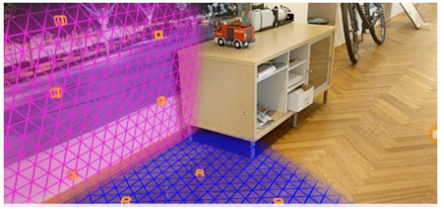
\includegraphics[width=.6\textwidth]{images/MobiDEV/4. augmented reality (display e interaction)/piano.PNG}
\end{center}


\begin{minipage}{.4\textwidth}
   In alcuni casi gli oggetti virtuali hanno significato solo in presenza di altri oggetti del mondo reale che possono essere sia 2D che 3D. Molte librerie di AR rendono disponibili delle funzioni per riconoscere dei template 2D ed anche in questo caso, la libreria di AR fornisce la posizione nello spazio di queste immagini, così da rendere possibile il disegno di altri oggetti virtuali. Un esempio ne è un sistema che riconosce un quadro e disegna una linea che evidenzia una parte di esso. 
\end{minipage} 
\hfill
\begin{minipage}{.6\textwidth}
    \begin{center}
        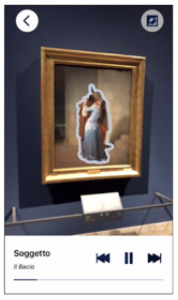
\includegraphics[width=.5\textwidth]{images/MobiDEV/4. augmented reality (display e interaction)/template 2D.PNG}
    \end{center}
\end{minipage}

\begin{minipage}{.6\textwidth}
    \begin{center}
        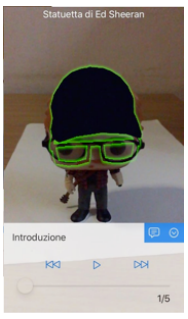
\includegraphics[width=.4\textwidth]{images/MobiDEV/4. augmented reality (display e interaction)/template 3D.PNG}
    \end{center}
\end{minipage}
\hfill
\begin{minipage}{.4\textwidth}
   Alcune librerie di AR (tra cui ARKit) permettono anche di riconoscere un template 3D.
   \\ L'app riconosce il template (la statuetta) fisico e disegna oggetti virtuali sopra di esso.
\end{minipage} 


Un altro problema è relativo alla sorgente luminosa. 
Dobbiamo identificare la sorgente luminosa per disegnare l'oggetto e per disegnare le ombre. 

\subsection{Problema dell'occlusione}
Il problema nasce quando dobbiamo far interagire il sistema reale con quello virtuale.
Si ha quindi il problema quando un oggetto fisico si frappone tra la camera e un oggetto virtuale, ma il sistema di AR non lo sa e disegna l'oggetto virtuale come se apparisse di fronte a quello reale.

Per risolvere il problema dell'occlusione è necessario comprendere se c'è un oggetto reale che si interpone tra la camera e un oggetto virtuale e capire esattamente dove si trova. In questo modo è possibile identificare quali parti dello schermo non debbano essere disegnate con gli oggetti virtuali.
Questo richiede delle capacità di riconoscere la distanza fisica degli oggetti dalla camera.

\subsection{Riconoscimento della scena}
Le librerie di AR rilasciano nuove funzionalità per riconoscere la scena. 
Questo sviluppo delle funzionalità procede di pari passo con la potenza computazionale dei device e con la disponibilità di nuovi sensori. 
Per esempio, grazie al lidar, ARKit riesce a riconoscere un insieme di oggetti. 

Ci sono casi in cui vorremmo togliere oggetti reali aggiungendo oggetti virtuali, ad esempio tolgo il mobile reale, per mettere quello virtuale dell'ikea. 
Il problema è che devo stimare cosa c'è dietro l'oggetto.  Attraverso l'uso di tecniche di machine learning si riesce a stimare l'immagine da mostrare sulla base di quella nota, ad esempio ripetendo un pattern noto sullo sfondo.

\section{Display audio}
L'audio può essere usato come componente di output di un sistema di AR:
\begin{itemize}
    \item in assenza di informazioni visive: es, in un sistema di supporto alle persone non vedenti 
    \item in combinazione ad informazioni visive, per dare maggiore realismo agli elementi virtuali 
\end{itemize}

L'audio si ottiene sfruttando un principio percettivo del suono. Percepiamo il suono in un modo diverso da un orecchio all'altro.
Le differenze tra i due canali possono essere:
\begin{itemize}
    \item interaural level difference (ILD): simulo una differenza di volume nell'orecchio destro e sinistro. Se c'è un suono a sinistra di una persona, la persona sentirà il volume del suono maggiore nell'orecchio sinistro
    \item interaural time difference (ITD): impostare una differenza di tempo nel canale. Se c'è un suono a sinistra di una persona, l'orecchio sinistro di quella persona riceverà il suono prima dell'orecchio destro
\end{itemize}

Conosciamo il suono nell'ambiente simulato, ma non conosciamo la propagazione del suono nell'ambiente reale e per questo ci sono diversi problemi: 
\begin{itemize}
    \item della posizione della testa: sappiamo com'è orientato il dispositivo ma non sappiamo com'è orientata la testa dell'utente. È rischioso assumere che l'utente sia orientato come il device (es: se gira la testa?). Si possono pensare varie soluzioni come l'uso di hardware posizionato sulla testa dell'utente, come ad esempio cuffie con sensori inerziali o il riconoscimento della posizione del volto rispetto al device (al momento non è possibile effettuare una sessione AR sia con la camera frontale che con quella posteriore)
    \item dell'ambiente: com'è l'ambiente virtuale per cercare di capire come si propaga il suono nel mondo reale. Lo stesso suono sarà percepito in modo differente cambiando l'ambiente (es indoor o outdoor). La comprensione dell'ambiente può aiutare a generare un suono più realistico
    \item anatomia dell'ascoltatore: la forma della testa e del torso impattano su come una persona percepisce il suono. Esistono dei modelli chiamati HRTF (Head Related Transfer Functions) che permettono di modellare come un utente percepisce il suono in base a molti fattori
\end{itemize}

\section{Interazione}
I sistemi di AR possono richiedere all'utente di interagire con oggetti reali e virtuali. 
Abbiamo due problemi: 
\begin{itemize}
    \item come selezionare un elemento del mondo 3D partendo dalle coordinate 2D dello schermo
    \item come permettere all'utente di manipolare oggetti nel mondo 3D
\end{itemize}

In entrambi i casi abbiamo coordinate schermo 2D e del mondo reale 3D. 
Quando abbiamo un oggetto virtuale 3D, ogni punto si rimappa in al più una coordinata dello spazio bidimensionale. 
Quando vogliamo la cosa inversa, abbiamo che in un punto 2D corrispondono infiniti punti nel mondo 3D che corrispondono a quel punto. 

Le librerie di AR rendono disponibile Hit test, una funzione che preso in input un punto delle coordinate schermo, ritorna l'elenco di tutti gli oggetti riconosciuti che sono toccati da questo raggio. 
si proietta una linea (chiamata raycast) che parte dal punto 2D indicato e si estende seguendo l'apertura focale della camera.
L'hit test ritorna l'elenco di oggetti intersecati.
\begin{center}
    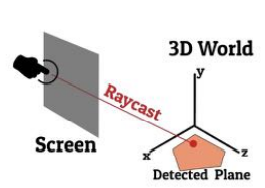
\includegraphics[width=.5\textwidth]{images/MobiDEV/4. augmented reality (display e interaction)/hit test.PNG}
\end{center}
           
Quando vogliamo manipolazione gli oggetti virtuali, abbiamo il problema della dimensionalità. 
Gli oggetti virtuali hanno 9DOF (posizione, rotazione e dimensione sui 3 assi) e devo capire come gestire questi 9 gradi. 
Ci sono due approcci principali:
\begin{itemize}
    \item integrality: l'utente può interagire con tutte le dimensioni in contemporanea
    \item separability: l'utente può manipolare una dimensione per volta
\end{itemize}

L'interazione con gli oggetti può avere 3 soluzioni:
\begin{itemize}
    \item tramite schermo: 
    \item tramite proxy fisici
    \item movimenti delle mani nello spazio
\end{itemize}

\subsection{Interazione tramite schermo}
Si può usare un approccio basato su integrality, perché possiamo usare gesti diversi per dimensioni diverse, ad esempio spostare un oggetto con tocco con due dita, cambiare la dimensione con il pinch ecc. Tuttavia questi gesti non sono standard e l'utente deve essere istruito su come fare.

Il problema è che con il tocco sullo schermo posso spostare a destra/sinistra, e in alto/basso, ma non posso avvicinare/allontanare l'oggetto. 
Le possibili soluzioni:
\begin{itemize}
    \item aggiunta di un controllo per la distanza: stiamo applicando il principio della separability
    \item faccio in modo che almeno una dimensione dell'oggetto virtuale sia vincolata al mondo fisico (es: l'oggetto non vola, ma è appoggiato per terra). In questo caso l'oggetto ha due gradi di libertà sulla posizione e lo posso riappare più facilmente sulle schermo
\end{itemize}

\subsection{Interagire tramite proxy fisici}
\begin{minipage}{.4\textwidth}
   Possiamo avere oggetti virtuali controllati tramite oggetti fisici, ad esempio spostiamo un oggetto virtuale spostando un marcatore esplicito.
   Un esempio potrebbe essere la bacchetta nell'immagine, che ha diversi marcatori aruco, grazie ai quali è possibile calcolare non solo la posizione ma anche la rotazione. 
   L'immagine è tratta da un sistema che permette di toccare un oggetto e capire quale oggetto è stato toccato. 
\end{minipage} 
\hfill
\begin{minipage}{.6\textwidth}
    \begin{center}
        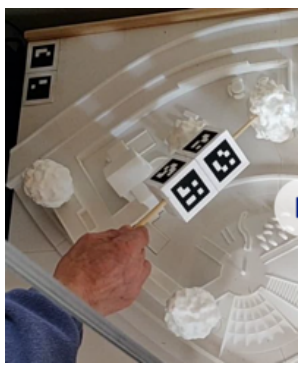
\includegraphics[width=.6\textwidth]{images/MobiDEV/4. augmented reality (display e interaction)/interazione tramite schermo.PNG}
    \end{center}
\end{minipage}

Le soluzioni basate su gesti sullo schermo sono limitate dal fatto che lo schermo è 2D, mentre lo spazio fisico è 3D. Un idea potrebbe essere che l'utente possa fare gesti direttamente nello spazio 3D in modo tale da rendere l'interazione più naturale, ad esempio “prendo” un oggetto virtuale con due dita e lo sposto/ruoto dove voglio.

